\section{Einleitung und Versuchsziel}
\label{sec:aufgabenstellung}
%In der Aufgabenstellung wird (in eigenen Worten und ganzen Sätzen) formuliert, was das Ziel des 
%Versuches ist.  
%[Beachten Sie die eigentliche Aufgabenstellung in den Versuchsanleitungen sowie die Hinweise zur Auswertung!] 

Im folgenden Versuch werden aus handelsübliche Nelkenblüten die ätherischen Öle extrahiert und charakterisiert. Wesentliche Arbeitsmethoden sind bei diesem Versuch die Wasserdampfdestillation, das Extrahieren, sowie das Rotationsverdampfen. Die ätherischen Öle der Nelken werden massenspektroskopisch per  Gaschromatografie analysiert.\\
Die Hauptkomponenten der ätherischen Öle der Nelke, die in diesem Versuch extrahiert wurden, wird nach Recherchen mit den Verbindungen \textit{Eugenol} und \textit{Eugenolacetat} beschrieben \cite{Berger.2017,Krammer.2003}.

\begin{figure}[h!]
	\centering
	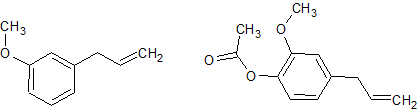
\includegraphics[width=0.9\textwidth]{img/Eugenol_Eugenolacetat.png}
	\caption{Strukturformeln der Verbindungen Eugenol und Eugenolacetat}
\end{figure}
\FloatBarrier
%Ende